\section{Anexos}

\subsection{Manual de usuario}
\label{manual-usuario}
\subsubsection{Menú de Navegación}

El menú de navegación es una de las partes más necesarias de aclarar, puesto que a través de él los usuarios pueden acceder a las diferentes secciones de la aplicación de manera sencilla e intuitiva. El menú está ubicado en la parte superior de la pantalla y contiene enlaces directos a las funcionalidades principales, como el inicio, rutas de viaje, configuración de perfil y vista de proveedor. Además, el menú es responsivo, adaptándose a distintos tamaños de pantalla para garantizar una experiencia óptima tanto en computadoras como en dispositivos móviles.

\vspace{2mm}
\begin{minipage}{0.9\textwidth}
\centering
\captionof{figure}[{Barra de navegación.}]{Barra de navegación.}
\label{ManualBarraNavegacion}
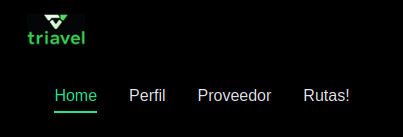
\includegraphics[width=0.7\textwidth]{Content/Images/ManualBarraNavegacion.png}
\footnote{Nota. \textup{Fuente: Autores.}}
\end{minipage}

La barra de búsqueda permite a los usuarios encontrar rutas, destinos o proveedores de manera rápida y eficiente. Al escribir una palabra clave en la barra de búsqueda, el sistema sugiere resultados relevantes en tiempo real, facilitando la navegación y el acceso a la información deseada. Esta funcionalidad mejora significativamente la experiencia del usuario al reducir el tiempo necesario para localizar opciones específicas dentro de la aplicación.

\vspace{2mm}
\begin{minipage}{0.9\textwidth}
\centering
\captionof{figure}[{Barra de búsqueda.}]{Barra de búsqueda.}
\label{ManualBarraBusqueda}

\includegraphics[width=0.7\textwidth]{Content/Images/ManualBarraBusqueda.png}
\footnote{Nota. \textup{Fuente: Autores.}}
\end{minipage}

Los botones principales de búsqueda para filtrar los restaurantes, hoteles y demás sitios turísticos ayudan a filtrar los espacios para que aparezcan de acuerdo a las necesidades del usuario.

\vspace{2mm}
\begin{minipage}{0.9\textwidth}
\centering
\captionof{figure}[{Botones de búsqueda.}]{Botones de búsqueda.}
\label{ManualBotonesBusqueda}
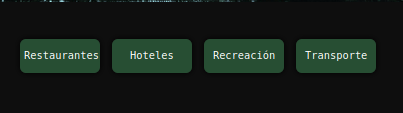
\includegraphics[width=0.7\textwidth]{Content/Images/ManualBotonesDeBusqueda.png}
\footnote{Nota. \textup{Fuente: Autores.}}
\end{minipage}

Los botones de carrusel permiten el desplazamiento entre los diferentes elementos dispuestos en carruseles, sean lugares, noticias o reseñas.

\vspace{2mm}
\begin{minipage}{0.9\textwidth}
\centering
\captionof{figure}[{Botones de carrusel.}]{Botones de carrusel.}
\label{ManualBotonesCarrusel}
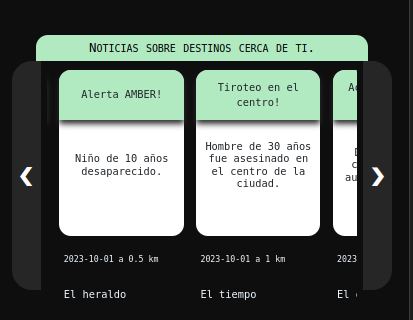
\includegraphics[width=0.7\textwidth]{Content/Images/ManualFlechasCarrusel.png}
\footnote{Nota. \textup{Fuente: Autores.}}
\end{minipage}

\subsection{Criterios de aceptación}

1. Las funcionalidades del aplicativo deben estar terminadas en un 90\% y probadas antes de finalizar el primer año de producción.

2. Pese a que se propone un margen de presupuesto destinado a riesgos, se espera que el desarrollo del proyecto no consuma la totalidad de este presupuesto; el criterio de aceptación, entonces, es que no consuma más del 60\% del presupuesto destinado a riesgos.

3. El aplicativo debe ser capaz de soportar un mínimo de 1000 usuarios concurrentes después del primer año de desarrollo sin degradar su rendimiento, garantizando una experiencia fluida y eficiente para todos los usuarios.

4. Se espera también que, como propuesta de negocio, el modelo haya captado como mínimo el estimado de clientes previsto para el primer año.

\subsection{Certificación de viabilidad de Parquesoft}
\centering
\captionof{figure}[{Carta de Parquesoft}]{Carta de Parquesoft}
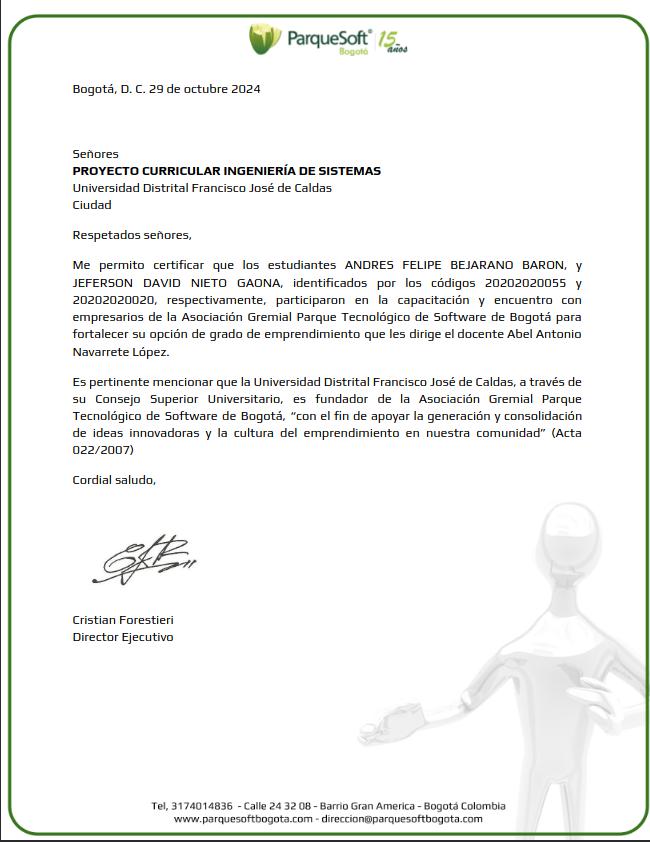
\includegraphics[width=0.7\textwidth]{Content/Images/CartaParquesoft.png}
\footnote{Nota. \textup{Fuente: Autores.}}
